\documentclass{article}
\usepackage[yyyymmdd]{datetime}
\usepackage[nottoc]{tocbibind}
\usepackage{xurl}
\usepackage{array}
\usepackage{float}
\usepackage[inline,shortlabels]{enumitem}
\usepackage{hhline}
\usepackage{multirow}
\usepackage{graphicx}
\usepackage{pgfplots}
\pgfplotsset{compat=1.18}
\usepackage[margin=1in]{geometry}
\usepackage[dvipsnames]{xcolor}
\usepackage{colortbl}
\usepackage[framemethod=TikZ]{mdframed}
\usepackage{amsfonts}
\usepackage{tikz}
\usepackage{amsthm}
\usepackage{amsmath}
\newtheoremstyle{problemstyle}{3pt}{3pt}{\normalfont}{}{\bfseries}{\normalfont\bfseries:}{.5em}{}
\theoremstyle{problemstyle}
\newmdtheoremenv[
  linewidth=1pt,
  linecolor=RoyalBlue,
  backgroundcolor=RoyalBlue!10,
  roundcorner=5pt,
  innertopmargin=6pt,
  innerbottommargin=6pt,
  innerleftmargin=6pt,
  innerrightmargin=6pt,
  nobreak=true
]{problem}{Problem}

% Example
\newmdtheoremenv[
  linewidth=1pt,
  linecolor=ForestGreen,
  backgroundcolor=ForestGreen!10,
  roundcorner=5pt,
  nobreak=true
]{example}{Example}

% Theorem
\newmdtheoremenv[
  linewidth=1pt,
  linecolor=BrickRed,
  backgroundcolor=BrickRed!10,
  roundcorner=5pt,
  nobreak=true
]{theorem}{Theorem}

% Remark
\newmdtheoremenv[
  linewidth=1pt,
  linecolor=Goldenrod,
  backgroundcolor=Goldenrod!10,
  roundcorner=5pt,
  nobreak=true
]{remark}{Remark}

% Solution
\newenvironment{solution}{%
  \begin{mdframed}[linewidth=0.8pt,linecolor=Gray,backgroundcolor=Gray!5,roundcorner=5pt]%
  \noindent\textbf{Solution.}%
}{%
\hfill $ \qed $ 
  \end{mdframed}%
}

\usepackage{listings}


% Make header with name and date etc.
\usepackage{fancyhdr}
\lhead{Pedro D. Llerenas\\An\'alisis de Datos I}
\rhead{\today\\Tarea III}
\thispagestyle{fancy}

\usepackage[utf8]{inputenc}
\setlength{\parindent}{0pt} % Don't indent new paragraphs
\setlength{\headheight}{24pt} 

\newcommand{\Z}{\mathbb Z}
\newcommand{\Q}{\mathbb Q}
\newcommand{\R}{\mathbb R}
\newcommand{\C}{\mathbb C}
\newcommand{\N}{\mathbb N}
\newcommand{\abs}[1]{\lvert #1 \rvert}
\DeclareMathOperator{\Var}{\mathbf{Var}}
\DeclareMathOperator{\E}{\mathbf{E}}


\begin{document}

%begin problem 1
\begin{problem}
Busca una variable aleatoria de la vida real que no es discreta ni continua.
\end{problem}
%end problem 1

%begin solution 1
\begin{solution}
	Sea $ X $ una v.a. representando el resultado de tirar una moneda justa. Sea $ Y $ (con $ X\perp Y $) una v.a. representando la distancia (en cm) del centro a un dardo tirado hacia una diana de radio 21cm. Asumimos que los dardos caen de manera uniforme en la diana. Sean $ Z $ (con $ X\perp Z $) los puntos que otorga la posici\'on en la que cae este dardo. Entonces, $ Y $ es una v.a. continua y $ Z $ es una v.a. discreta, que solo toma los puntos otorgados por regi\'on. Asumimos que cada regi\'on que divide la diana es de area similar, de esta manera, todos las regiones tienen probabilidad similar ($ 1/82 $).
	\begin{figure}[H]
		\centering
		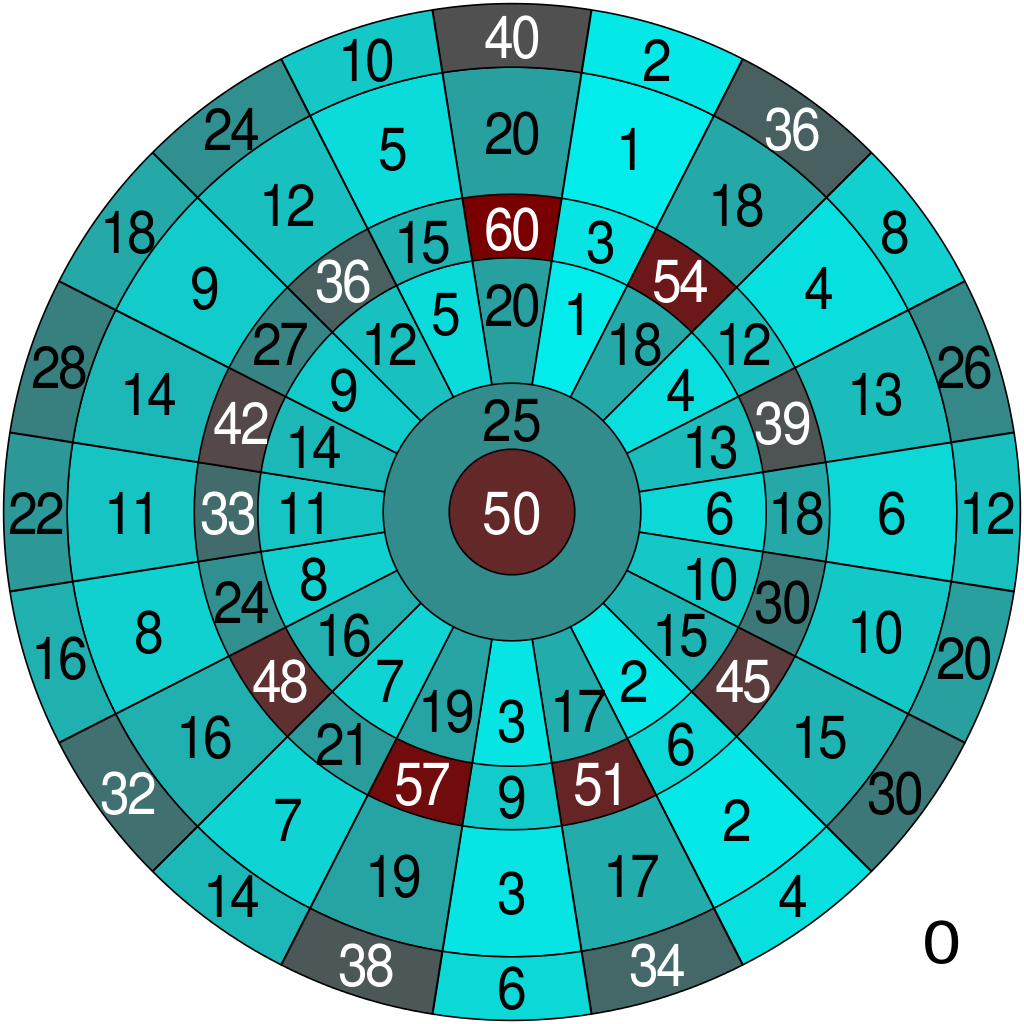
\includegraphics[scale=0.1]{images/Dartboard_heatmap.png}
		\caption{Ejemplo de diana con puntuaciones.}
	\end{figure}
	Definimos una nueva v.a.
	\begin{align*}
		M = \begin{cases}
			    Z & \text{ if }X = 0, \\
			    Y & \text{if } X = 1.
		    \end{cases}
	\end{align*}
	Notemos entonces que, por definici\'on,
	\begin{align*}
		F_M(x) & = P(M\leq x)                                     \\
		       & = \frac{1}{2}P(Y\leq x) + \frac{1}{2} P(Z\leq x) \\
		       & = \displaystyle\frac{F_Y(x) + F_Z(x)}{2},
	\end{align*}
	Sin embargo, esta suma no es continua ni discreta. Podemos observar esto cerca de $ x = 1 $: sea $ \varepsilon > 0 $, entonces
	\begin{align*}
		F_M(1-\varepsilon) & = \frac{(1-\varepsilon)^2}{2\cdot 21^2} + 0  \\
		F_M(1)             & = \frac{1}{2\cdot 21^2} + \frac{1}{2\cdot 2}
	\end{align*}
	Es decir, tenemos una discontinuidad en $ x=1 $. No es discreta porque es continua en $ x\in (1,2) $.

\end{solution}
%end solution 1

\pagebreak
%begin problem 2
\begin{problem}
El tiempo de ejecuci\'on (en segundos) de un cierto programa de optimizaci\'on tiene densidad:
\begin{align*}
	f_{X}(x) = c(0.4x^2 + x) \qquad \text{si } x\in [1,10].
\end{align*}
Calcula el valor de la constante y dibuja la densidad.

Supongamos que se dice que el programa es exitoso si el tiempo de ejecuci\'on es menos de 6 segundos. Al correr el programa 20 veces, suponiendo que las corridas son independientes, calcula la probabilidad de tener menos de 8 corridas exitosas.
\end{problem}
%end problem 2

%begin solution 2
\begin{solution}
	Recordemos que una funci\'ion de densidad debe cumplir, para todo $ x\in \Omega $,
	\begin{enumerate}[a)]
		\item $ f_X(x)\geq 0 $,
		\item $ \int_{\Omega} f_X(x) = 1 $
	\end{enumerate}
	En particular, b) nos dice que, en este caso, se debe cumplir
	\begin{align*}
		\int_{[1,10]} c(0.4x^2 + x)\,dx = 1 & \iff \int_{1}^{10} 0.4x^2 + x \,dx = c^{-1}.
	\end{align*}
	Entonces, resolvemos la integral:
	\begin{align*}
		\int_{1}^{10} 0.4x^2 + x \,dx & = \left[\frac{2}{5}\cdot\frac{x^3}{3} + \frac{x^2}{2}\right]_{1}^{10}                                                       \\
		                              & = \left[\frac{2}{5}\cdot\frac{10^3}{3} + \frac{10^2}{2}\right] - \left[\frac{2}{5}\cdot\frac{1^3}{3} + \frac{1^2}{2}\right] \\
		                              & =\frac{1827}{10} = 182.7.
	\end{align*}
	Entonces, $ c = \frac{10}{1827}\approx 0.0055 $.
	\begin{figure}[H]
		\centering
		\begin{minipage}{0.4\textwidth}
			\begin{tikzpicture}[scale=0.5,domain=1:10, xscale=0.5, yscale=20]
				\draw[very thin,color=white] (0,0) grid (10,0.3);

				\draw[->] (0,0) -- (12,0) node[right] {$x$};
				\draw[->] (0,0) -- (0,0.3) node[above] {$f_{X}(x)$};

				\draw[color=blue] plot (\x,{0.005*(0.4*\x*\x + \x)}) node[right] {$f_X(x)$};

				\draw (1, 0.005) -- (1, -0.005) node[below=4mm] {$1$};
				\draw (0.1,0.007) -- (-0.1, 0.007) node[left=4mm] {$0.007$};

				\draw (10, 0.005) -- (10, -0.005) node[below=4mm] {$10$};
				\draw (0.1,0.27) -- (-0.1, 0.27) node[left=4mm] {$0.27$};

			\end{tikzpicture}
		\end{minipage}
		\begin{minipage}{0.4\textwidth}
			\begin{tikzpicture}[scale=0.5,domain=1:10, xscale=0.5, yscale=0.1]
				\draw[very thin,color=white] (0,-0.1) grid (12,50);

				\draw[->] (0,0) -- (12,0) node[right] {$x$};
				\draw[->] (0,-0.2) -- (0,55) node[above] {$y$};

				\draw[color=blue] plot (\x,{0.4*\x*\x + \x}) node[right] {$0.4x^2 + x$};

				\draw (1, 0.5) -- (1, -0.5) node[below=4mm] {$1$};
				\draw (0.1,1.4) -- (-0.1, 1.4) node[left=4mm] {$1.4$};

				\draw (10, 0.5) -- (10, -0.5) node[below=4mm] {$10$};
				\draw (0.1, 50) -- (-0.1, 50) node[left=4mm] {$50$};
			\end{tikzpicture}
		\end{minipage}
		\caption{Funci\'on de distribuci\'on.}\label{fig:dist_f_p2}
	\end{figure}
	\hfill $\triangle$


	Para la segunda parte del ejercicio, primero notemos que
	\begin{align*}
		P(X\leq 6) & = c\int_{1}^{6}0.4x^2+x\,dx                                                                          \\
		           & = c\left[0.4 \frac{x^3}{3} + \frac{x^2}{2}\right]_{1}^{6}                                            \\
		           & = c\left[0.4 \frac{6^3}{3} + \frac{6^2}{2}\right] -  c\left[0.4 \frac{1^3}{3} + \frac{1^2}{2}\right] \\
		           & = c\left[0.4\cdot 72 + 18\right] -  c\left[0.4 \frac{1}{3} + \frac{1}{2}\right]                      \\
		           & \approx 46.166\cdot c                                                                                \\
		           & \approx 0.25.
	\end{align*}
  Ahora, sea $ Y $ el n\'umero de ejecuciones exitosas dentro de las 20 ejecuciones. Sea $ p = P(X\leq 6) $, entonces tenemos que $ Y\sim Bin(20, p) $. Podemos concluir que
  \begin{align*}
    P(Y\leq 7) &= \sum_{i=1}^{7} P(X=i)\\
               &= \sum_{i=1}^{7}\binom{20}{i}(1-p)^{20-i}p^{i}\\
               &\approx 0.895.
  \end{align*}

\end{solution}
%end solution 2

%begin problem 3
\begin{problem}
Se elige al azar un punto $ (X,Y) $ adentro del siguiente tri\'angulo.
\begin{figure}[H]
	\centering
	\begin{tikzpicture}
		\draw[step=1cm, gray!50,very thin] (-2.5, -0.5) grid (2.5, 5.5);
		\draw[thick] (-2.5,0) -- (2.5,0);
		\draw[thick] (0,-0.5) -- (0,5.5);
		\foreach \x in {-2,-1, 0,1,2}
		\draw[thin] (\x,0.1) -- (\x,-0.1) node[below right] {\tiny\x};

		\foreach \y in {1,2,3,4,5}
		\draw[thin] (0.1,\y) -- (-0.1,\y) node[above left] {\tiny\y};

		\draw[color=orange, very thick] (0,4) -- (2,0) -- (-2,0) -- (0,4);
		\draw[fill=blue, thick] (-2,0) circle (2pt) node[above left] {B};
		\draw[fill=blue, thick] (2,0) circle (2pt) node[above right] {C};
		\draw[fill=blue, thick] (0,4) circle (2pt) node[above right] {A};
	\end{tikzpicture}
	\label{tikz:trinagle}
\end{figure}
Calcula
\begin{enumerate}[a)]
	\item $ P(|X| < 0.1) $,
	\item $ \displaystyle\int_{-2}^{2}x f_X(x)\,dx $.
\end{enumerate}
\end{problem}
%end problem 3

%begin solution 3
\begin{solution}
	\begin{enumerate}[a)]
		\item $ P(|X| < 0.1) $,
		      Podemos interpretar el tri\'angulo de la siguiente manera:
		      \begin{align*} y =
			      \begin{cases}
				      2x+4,  & \text{ if } -2\leq x < 0    \\
				      -2x+4, & \text{ if } 0 \leq x \leq 2 \\
				      0      & \text{ otherwise}
			      \end{cases}
		      \end{align*}
		      O de manera equivalente, $ y = -2|x|+4 $ para $ x\in [-2,2] $.
		      El \'area del tri\'angulo es $ 4\cdot4/2 =8$, por lo que podemos decir que la funci\'on de distribuci\'on est\'a dada por $ f_X(x) = \frac{1}{8}(-2|x|+4) $. Entonces, tenemos
		      \begin{align}
			      8\cdot P(|X|<0.1) & = \displaystyle\int_{-0.1}^{0.1}-|2x|+4\,dx\nonumber    \\
			                        & =2\int_{0}^{0.1} -|2x|+4\,dx\label{eq:1}                \\
			                        & =2\int_{0}^{0.1} -2x+4\,dx                 \label{eq:2} \\
			                        & =2\left[-x^2+4x\right]_{0}^{0.1}            \nonumber   \\
			                        & =2(0.4-0.01)                               \nonumber    \\
			                        & =0.78.\nonumber
		      \end{align}
		      donde \eqref{eq:1} se sigue del hecho de que $ -2|x|+4 $ es una funci\'on par, y \eqref{eq:2} de que $ |x| = x $ si $ x\geq 0 $.

		      Es decir, $ P(|X|<0.1) = 0.78/8 = 0.0975 $.\hfill$\triangle$
		\item $ \displaystyle\int_{-2}^{2}x f_X(x)\,dx $
		      En el inciso anterior descubirmos que
		      \begin{align*}
			      f_X(x) =
			      \begin{cases}
				      \frac{-2|x|+4}{8}, & \text{ if }x\in [-2,2] \\
				      0,                 & \text{ otherwise}
			      \end{cases}
		      \end{align*}
		      Por lo que tenemos que
		      \begin{align}
			      \int_{-2}^{2}x f_X(x)\,dx & = 0,\label{eq:3}
		      \end{align}
		      donde \eqref{eq:3} se sigue del hecho de que $ xf_X(x) $ es una funci\'on (integrable) impar (ya que $ f_X(x) $ es par, y $ x $ es impar), siendo integrada sobre un intervalo sim\'etrico.
	\end{enumerate}
\end{solution}
%end solution 3
\pagebreak
%begin problem 4
\begin{problem}
Cada vez cuando uno compra una bolsa de Sabritas, se recibe una foto de uno de los 20 jugadores de los Diablos Rojos. Si las fotos son distribuidas de una manera arbitraria en las bolsas, calcula el promedio del n\'umero de bolsas que uno va tener que comprar para obtener una foto que no sea la del jugador Romelu Lukaku.

¿En promedio cu\'antas bolsas vas a tener que comprar para tener todos los 20 jugadores?
%end problem 4
\end{problem}

%begin solution 4
\begin{solution}
	Sea $ X $ la cantidad de bolsas que debemos comprar para obtener una foto distinta a la Romelu Lukaku. Como son distribuidas de manera arbitraria (y que hay un n\'umero infinito de bolsas), la probabilidad de obtener una foto que no sea de Romelu Lukaku es de $ 19/20 $. Es decir, la probabilidad de un \'exito es de $ 19/20 $, por lo que $ X\sim Geom(19/20) $, por lo que
	\begin{align*}
		\E[X] = \frac{20}{19} \approx 1.05.
	\end{align*}

  Ahora, sean $ Y_0,\dots,Y_{19} $ v.a. indicando la cantidad de bolsas para obtener el jugador $ i $ por primera vez. Entonces, $ Y_i\sim Geom(1/20) $. Sea $ Z $ la v.a. indicando las bolsas a compara para conseguir los 20 jugadores, entonces tenemos que $ Z = \sum Y_i $. Por linealidad, tenemos
  \begin{align*}
    \E[Z] = \sum_i \E[Y_i] = 20.
  \end{align*}
\end{solution}
%end solution 4

\bibliographystyle{plain}
\bibliography{references}

\end{document}
